\chapter{幾何学、情報、そしてブラックホールの面積則}

\lectureoverview{宣言された目的地は宇宙論であるが、そこへの最短の道は特殊相対性理論への回帰から始まる。計量は時空の幾何学を教え、固有時間がゼロであるという条件は光がどのように運動するかを教える。この一つの規則をシュヴァルツシルト幾何学へと持ち込み、事象の地平面と特異点を区別し、そしてブラックホールが放射によって蒸発するとき情報はどうなるのかを問う。その答えは通常のエントロピーから始まり、ベッケンシュタインの1ビットの議論で終わる。すなわち、ブラックホールは体積ではなく地平面の面積を単位として情報を蓄えるのである。}

ススキンドは、弦理論の成功と失敗について約束した会計をしばらく延期する。彼によれば、時間が遅く、また監査よりも実質の方が有用である。今夜の実質とは、ブラックホール情報問題を定式化するために必要な最小限の幾何学と熱力学である。

\section{光に対する一つの規則}

特殊相対性理論は空間と時間を一つの幾何学的対象として扱う。\(dt,dx,dy,dz\)だけ離れた隣接する事象に対して、ススキンドは主にマイナスの符号の規約を用いて次のように書く。
\begin{equation}
d\tau^2=dt^2-\frac{1}{c^2}\left(dx^2+dy^2+dz^2\right).
\end{equation}
時間的部分と空間的部分の符号が反対であることが、ミンコフスキー幾何学を4次元ユークリッド幾何学から区別する。因子\(1/c^2\)は単に単位を調和させるだけであり、時間と距離を整合的に測ることにより\(c=1\)と置くことができる。

時間的隔たりでは\(d\tau^2>0\)であり、\(d\tau\)はその軌道に従う時計が記録する固有時間である。空間的隔たりでは代わりに\(d\tau^2<0\)となる。今夜必要となる場合はちょうどその中間にある。光線は\emph{ヌル}な軌道に従い、
\begin{equation}
d\tau^2=0.
\end{equation}
まず\(x\)軸に沿った運動に制限すると、
\begin{align}
0&=dt^2-\frac{dx^2}{c^2},\\
c\,dt&=\pm dx,\\
\frac{dx}{dt}&=\pm c.
\end{align}
符号は右向きおよび左向きの光線を表す。\(c\)に割り当てられる数値は、センチメートルをメートルやキロメートルに置き換えると変化する。不変な言明は数ではなく、ヌル条件である。

一般相対性理論が複雑にするのは計量であって、この規則ではない。座標\(x^\mu\)、\(\mu=0,1,2,3\)を用いると、
\begin{equation}
ds^2=g_{\mu\nu}(x)\,dx^\mu dx^\nu,
\end{equation}
ここで繰り返された添字は和をとり、係数は点ごとに変化しうる。光が局所的に許される方向を見つけるには、この二次形式をゼロと置けばよい。

\section{球座標とシュヴァルツシルト計量}

回転しないブラックホールは球対称であるため、デカルト座標は有用な構造を隠してしまう。\(r\)を動径距離とし、\(\theta,\phi\)を単位球面上の方向を指定するものとしよう。その線素は
\begin{equation}
d\Omega^2=d\theta^2+\sin^2\theta\,d\phi^2.
\end{equation}
である。半径\(r\)の球面上では、角度の変位はしたがって\(r^2d\Omega^2\)に寄与する。球座標における平坦な時空は
\begin{equation}
d\tau^2=dt^2-\left(dr^2+r^2d\Omega^2\right),
\qquad (c=1).
\end{equation}
である。

ススキンドはアインシュタイン方程式からブラックホール解を導出しない。彼はそれを書き下し、我々にそれを吟味するよう求める。黒板は意図された比較を明示する。

\begin{figure}[htbp]
\centering
\includegraphics[width=0.86\textwidth]{lecture_02_figure_02.png}
\caption{上は平坦な球面時空、下はシュヴァルツシルトの変形。繰り返される因子\(1-2GM/(c^2r)=1-R_s/r\)と動径方向のスケッチが一緒に見える。}
\lectureframe{00:19:12.520}
\end{figure}

質量\(M\)のブラックホールに対して、シュヴァルツシルト半径を
\begin{equation}
R_s=\frac{2GM}{c^2}.
\end{equation}
と定義する。外部の線素は
\begin{equation}
d\tau^2=\left(1-\frac{R_s}{r}\right)dt^2
-\frac{dr^2/c^2}{1-R_s/r}
-\frac{r^2}{c^2}d\Omega^2.
\label{eq:schwarzschild-explicit-c}
\end{equation}
である。等価に、\(c=1\)と置いた後では、
\begin{equation}
ds^2=\left(1-\frac{2GM}{r}\right)dt^2
-\frac{dr^2}{1-2GM/r}-r^2d\Omega^2.
\label{eq:schwarzschild}
\end{equation}
となる。遠方では\(R_s/r\ll1\)であり、平坦な球面計量が戻ってくる。この漸近的検査は公式を暗記することよりも重要であるが、ススキンドは後者をカクテルパーティーの材料として推奨している。

\editorialnote{黒板は\(d\tau^2\)と\(ds^2\)の間で交互に切り替わり、\(c\)のすべての因子を一貫して表示しているわけではない。式~\eqref{eq:schwarzschild-explicit-c}は講義の時間座標の規約に従っており、そこでは\(t\)は時間の単位を持つ。\(x^0=ct\)を用いた標準的な形は代数的に等価である。}

\subsection{地平面は特異点ではない}

座標の中で二つの半径が怪しく見える。自然単位で\(r=R_s=2GM\)では、\(dt^2\)の係数が消え、\(dr^2\)の係数が発散する。\(r=0\)では、曲率自体が特異になる。これらは同じ事象の二つの版ではない。
\begin{equation}
\begin{aligned}
r=R_s &:\quad \text{horizon},\\
r=0 &:\quad \text{curvature singularity}.
\end{aligned}
\end{equation}

潮汐力が物理的な区別を与える。重力場は広がりを持つ物体の各部で異なる。すなわち、足は頭よりも強く引かれ、物体を引き伸ばす一方で横方向は圧縮される。地平面ではそれらの潮汐力は有限であり、十分に大きな質量のブラックホールの地平面では非常に小さくなりうる。そこでは局所的に破局的なことは何も起こる必要がない。対照的に\(r=0\)では、潮汐力は発散する。\(r=R_s\)における警告的な係数はシュヴァルツシルト座標の欠陥を告げている。\(r=0\)の特異点は物理的である。

\editorialnote{曲率が\(r=R_s\)で有限であることは、Kretschmannスカラー\(R_{\mu\nu\rho\sigma}R^{\mu\nu\rho\sigma}=48G^2M^2/(c^4r^6)\)から確認できる。これは事象の地平線で有限であり、\(r\to0\)でのみ発散する。この不変量は講義では書かれなかったが、潮汐力の区別を精密にするものである。}

\section{地平線近傍の動径方向の光}

ここで一つの規則に戻る。動径方向の光線は角位置を固定したままであるから、\(d\Omega=0\)であり、光線では\(ds^2=0\)である。\(c=1\)単位では、式~\eqref{eq:schwarzschild}より
\begin{equation}
0=\left(1-\frac{2GM}{r}\right)dt^2
-\frac{dr^2}{1-2GM/r}.
\end{equation}
\(1-2GM/r\)を掛けて平方根をとると二つの分枝が得られる。
\begin{align}
dr&=\pm\left(1-\frac{2GM}{r}\right)dt,\\
\frac{dr}{dt}&=\pm\left(1-\frac{2GM}{r}\right).
\label{eq:radial-null}
\end{align}
プラス符号は外向き、マイナス符号は内向きである。遠方ではそれらの座標速度は\(\pm1\)に近づく。地平線では両者とも\(\lvert dr/dt\rvert\to0\)を満たす。すなわち、Schwarzschild座標時間では、外向き光線はそこで静止しているように見え、内向き光線は到達するのに無限の座標時間を要する。

\begin{figure}[htbp]
\centering
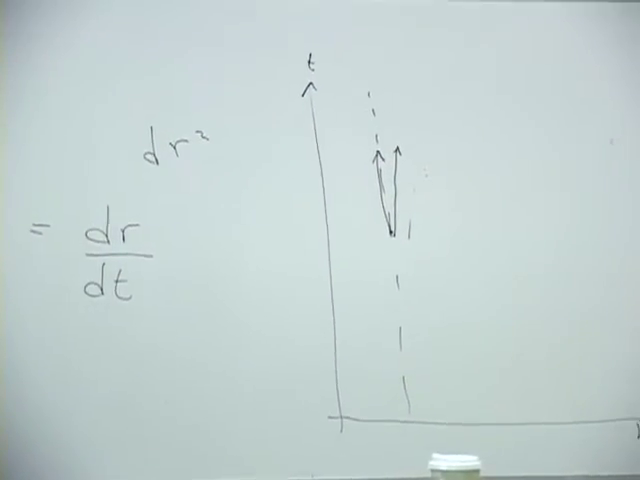
\includegraphics[width=0.82\textwidth]{lecture_02_figure_03.png}
\caption{完成した\(t\)-\(r\)黒板スケッチ。破線の地平線に近づくにつれて、動径方向のヌル光線はほぼ垂直になる。}
\lectureframe{00:30:25.000}
\end{figure}

\begin{figure}[htbp]
\centering
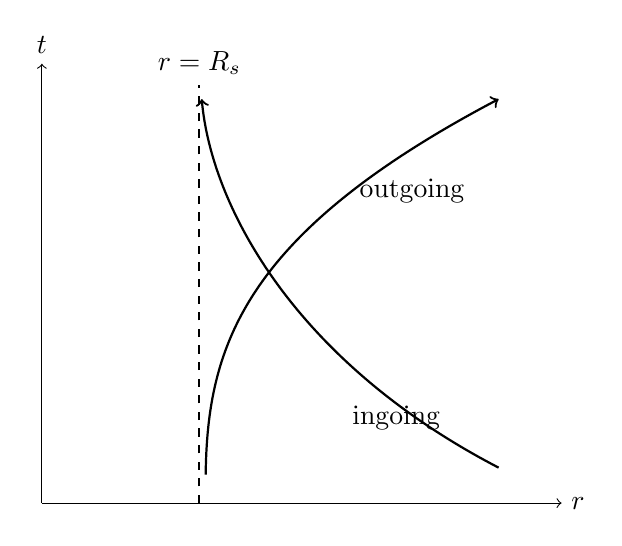
\begin{tikzpicture}[x=1.0cm,y=0.9cm]
\draw[->] (0,0) -- (6.6,0) node[right] {$r$};
\draw[->] (0,0) -- (0,6.2) node[above] {$t$};
\draw[dashed,thick] (2.0,0) -- (2.0,5.9) node[above] {$r=R_s$};
\draw[thick,->] (2.08,.4) .. controls (2.10,2.2) and (2.55,3.8) .. (5.8,5.7);
\draw[thick,->] (5.8,.5) .. controls (3.2,2.0) and (2.15,4.2) .. (2.03,5.7);
\node[align=center] at (4.7,4.4) {outgoing};
\node[align=center] at (4.5,1.2) {ingoing};
\end{tikzpicture}
\caption{黒板スケッチを座標時間で整理した版。見かけの減速はSchwarzschild\(t\)についての記述であり、光が\(c\)で進むことの局所的な破綻についてのものではない。}
\end{figure}

地平線の内側では、未来光円錐が内側へ大きく傾き、未来向きの動径方向の両分枝が\(r\)の減少へ向かう。そこから出発した信号は外部へ脱出できず、未来向きの因果的経路はすべて特異点に到達する。

\begin{classroomqa}
\audiencequestion{光速度が不変であるなら、地平線近くで光が減速すると言うことは正確には何を意味するのか。\lecturetimestamp{00:31:44}}
\lecturerresponse{表示された量は、特定の座標系における\(dr/dt\)である。数値的な速度は、メートルをセンチメートルに置き換えただけでもすでに変化する。ここでは、有効な動径方向と時間方向の目盛りが位置によって変わる。普遍的な言明は、すべての光線がヌル軌道\(ds^2=0\)に従うということである。}
\end{classroomqa}
\editorialnote{自由落下する局所観測者は真空中の光を\(c\)と測定する。地平線でSchwarzschild座標速度が消えることは局所的な観測量ではない。}

\begin{classroomqa}
\audiencequestion{光が通る物質媒質にかかわらず、同じヌル速度の言明が成り立つのか。\lecturetimestamp{00:33:24}}
\lecturerresponse{成り立たない。利用可能な認識は、もはやこの答えの説明を保持していない。}
\end{classroomqa}
\editorialnote{ヌル速度の主張は、真空時空における伝播に関するものである。物質との相互作用は波束に小さな有効速度を与えうるが、それは媒質の性質であり、局所的な因果速度\(c\)の変化ではない。}

\begin{classroomqa}
\audiencequestion{同じ\(t\)-\(r\)図で、入射する光線はどのように見えるか。\lecturetimestamp{00:33:32}}
\lecturerresponse{それは逆向きに見える分枝である。大きな\(r\)から地平線へ曲がり、漸近的に近づく。到達するには無限の座標時間\(t\)を要する。}
\end{classroomqa}
\editorialnote{落下する観測者は有限の固有時間で地平線に到達し、それを横切る。発散するのはSchwarzschild\(t\)のみである。}

\section{なぜ蒸発が問題を生むのか}

地平線はさらに多くの研究に値する。どのように形成されるか、落下する観測者に何が見えるか、そこで局所的に異常なことが起こるかどうかである。Susskindはこれらの問いを後回しにし、量子力学へと跳ぶ。外部から見ると、物質とその識別情報のすべてはますます地平線近くに押し込められ、利用できなくなる。それだけでは情報を破壊する必要はない。単に隠しているだけかもしれない。

Hawkingの結果はこの問題を深刻にする。落ち着いた古典的黑洞は、想像しうる最も退屈な物体のように見える。球対称で、暗く、メッセージを送ることができない。しかし``black''には二つの意味がある。何も放出しないという意味にもなりうるし、熱的な黒体放射を放出するという意味にもなりうる。量子的な黑洞は第二の意味で黒い。温度を持ち、輝き、エネルギーを失う。
\begin{equation}
E=Mc^2,
\qquad
R_s=\frac{2GM}{c^2},
\end{equation}
であるから、放射はその質量と地平線半径の両方を減少させる。蒸発が最終的に黑洞を消し去るなら、その地平線に残っているように見えた情報はどうなるのか。それは破壊されるか、小さな残骸に閉じ込められるか、外向き放射に符号化されるかもしれない。これらの可能性の間の緊張が情報問題であり、弦理論は後にその解決を鋭くする助けとなるであろう。

今夜は曲がった時空における量子場の計算は試みない。代わりにSusskindはBekensteinのより単純な道をたどる。まずエントロピーを情報として理解し、次に黑洞がどれだけの情報を隠せるかを計算する。

\section{存在するが隠されている情報}

箱を、各セルが占有されているか空であるかのどちらかになるほど小さなセルに分割することを想像しよう。二値文字列---セルごとに一つの答え---は、その配置を他のすべての許された配置から区別する。より現実的な物質では、粒子の種類や他の自由度についての問いが必要になるが、原理は変わらない。情報は、状態を指定するために必要なはい--いいえの問いの最小数によって測られる。

\begin{classroomqa}
\audiencequestion{これは静的な系の記述にすぎないのですか。\lecturetimestamp{00:45:49}}
\lecturerresponse{これはある1つの時刻における瞬間的な記述である。その後、力学がその状態を別の状態へ写す。}
\end{classroomqa}

次の原理はより深い。閉じた系の時間発展は、2つの異なる微視的状態を1つに融合しない。2つの配置が現在異なっているなら、それらが時間発展した配置も原理的には区別可能なままである。古典的ハミルトン時間発展は可逆であり、量子時間発展はユニタリである。\editorialnote{散逸的な有効方程式が区別を消し去ることができるのは、観測されない環境の自由度が省略されているからにすぎず、完全な閉じた状態はそれらを保持している。}

浴槽は、損失と到達不能性の違いを具体的にする。2つの水滴の流れは、2つの異なるモールス符号のテキストを符号化しうる。水が落ち着いた後、両方の浴槽は同じに見える。目に見える波紋は消えたが、完全な微視的測定を行えば、依然として異なる分子配置が見出されるであろう。メッセージは、追跡するには小さすぎ、多すぎる自由度へと広がってしまったのである。

エントロピーとは、この隠れた情報のことである。我々が問うことのできる巨視的な問い---温度、全エネルギー、組成、水位---に対して、多くの微視的区別は可能なままだが到達不能である。講義のビット数え上げの言葉では、
\begin{equation}
S=\hbox{number of hidden bits}.
\end{equation}
厳密な統計的公式は\(S=k_B\ln\Omega\)であるが、定性的な定義でブラックホールの議論には十分である。

\section{ビットを隠すコストとしての温度}

温度は測定するのは身近だが、定義するのは驚くほど間接的である。サスキンドはエントロピーとエネルギーを原始的な概念として選ぶ。コンピュータのビットが標準的な値にリセットされると仮定しよう。物理的デバイスは残るが、以前の0と1の状態の区別はコンピュータから消える。それは完全な世界から消えることはできず、環境の微視的自由度に移され、それらをわずかに加熱する。これがランダウアーの原理である。

1エントロピー単位が1ビットであり、温度がエネルギー単位で測られるなら、講義は次のように書く。
\begin{align}
\Delta S&=1,\\
\Delta E&=T\,\Delta S,\\
dE&=T\,dS.
\label{eq:first-law}
\end{align}

\begin{figure}[htbp]
\centering
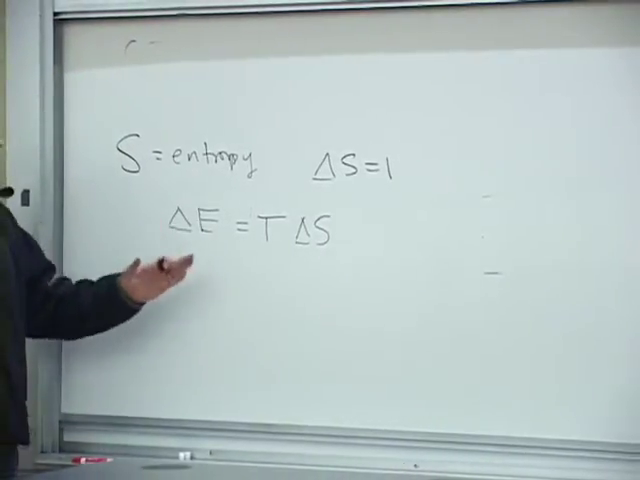
\includegraphics[width=0.84\textwidth]{lecture_02_figure_04.png}
\caption{黒板の情報理論的热力学：\(S\)はエントロピーであり、1つの隠れたビットは\(\Delta S=1\)を持ち、その最小エネルギーコストは\(\Delta E=T\Delta S\)と書かれる。}
\lectureframe{00:58:40.000}
\end{figure}

\editorialnote{従来の単位では、1つの二進ビットの可逆的消去コストは\(k_BT\ln2\)である。式~\eqref{eq:first-law}は\(k_B=1\)を用い、講義のエントロピー単位を1ビットとして扱い、関連する\(\ln2\)を抑制している。これらの規約は、続くスケーリングの議論には影響しない。}

ある聴衆による見積もりでは、およそ\(100\)ギガバイトを消去することによる最低温度上昇は、コップ一杯の水でおよそ\(10^{-15}\)度である。サスキンドは正確な数値ではなく、その要点を受け入れる。室温では1ビットが運ぶ最小エネルギーは極めて小さく、実際のコンピュータは消去が可逆的に行われないためにはるかに多くを散逸する。

\begin{classroomqa}
\audiencequestion{ハードドライブの例は単なる類推なのか、それとも消去による加熱は実際の法則なのか。\lecturetimestamp{01:00:02}}
\lecturerresponse{それは実際の物理的制約、すなわちランダウアーの規則である。メモリセルをリセットすると、古い区別がコンピュータから取り除かれ、その情報は環境へ運ばれなければならない。通常の操作は、回路を駆動し、電荷を移動させ、無関係な熱を生み出すため、理想的な最小値よりもはるかに効率が悪い。}
\end{classroomqa}

\begin{classroomqa}
\audiencequestion{1ビットを隠すコストは、より高い温度ではより多くのエネルギーを要しますか。\lecturetimestamp{01:02:07}}
\lecturerresponse{はい。関係\(dE=T\,dS\)はまさにそのことを述べている。同じエントロピー移動に対して、より熱い熱浴はより大きなエネルギー移動を必要とする。この隠れたビットあたりのエネルギー関係を温度の定義と見なすことも同様にできる。}
\end{classroomqa}

\begin{classroomqa}
\audiencequestion{以前に保存されたビットに上書きした場合、その古い情報は失われたのですか。\lecturetimestamp{01:02:43}}
\lecturerresponse{それはコンピュータから去ったが、閉じた物理系から消え去ったわけではない。上書きされた区別は環境へと分散され、そこで到達不能な情報として寄与し、したがってエントロピーに寄与する。}
\end{classroomqa}

熱力学的エントロピーを失われた微視的情報と同一視する見方はボルツマンにさかのぼる。シャノンは20世紀に対応する情報理論的な言語を与えた。ススキンドは、彼と聴衆の一部が1950年代に出会った熱力学の講義では、この説明が不思議なほど欠けていたと述べている。計算機科学によってこの結びつきは見落としにくくなったが、その物理的内容を生み出したわけではない。

\section{ブラックホールに1ビットを入れる}

今や、浴槽に一滴ずつ水を注ぐように、概念上ビットを一つずつ加えてブラックホールを構成できる。問題は微分形である。追加の1ビットが隠されたとき、事象の地平面はどれだけ成長するか。質量\(M\)、半径\(R_s\)の穴から始め、回収可能な区別が吸収されたかどうかだけである最も単純な物体を送り込む。

\begin{classroomqa}
\audiencequestion{情報が穴に入るには無限の座標時間が必要ではないのか。\lecturetimestamp{01:08:07}}
\lecturerresponse{それは地平面近傍で指数的に圧縮され、実際の短い時間のうちに外部から利用できなくなる。ただしシュヴァルツシルト座標時間では実際の横断に無限の値が割り当てられる。したがって外部の会計としては、地平面に蓄えられているとみなしてよい。}
\end{classroomqa}

光子は自然な候補であるが、一般的な光子は一ビットより多くの情報を運ぶ。その偏光は二値的な選択を符号化しうる。鋭く局在した到達点は、さらに多くのイエス--ノーの問いを与える。上半球か下半球か、左半分か右半分か、などである。量子力学は局在をおよそ一波長に制限するので、位置情報を抑える方法は、穴がなお吸収できる最長の波長を用いることである。

\begin{classroomqa}
\audiencequestion{光子が入ることのできない上限波長が本当にあるのか。\lecturetimestamp{01:12:15}}
\lecturerresponse{はい。穴よりずっと大きな波は、吸収されるよりも主に散乱される。有用な限界的選択は、地平面半径と同程度の波長である。すなわち、入射点をぼかすのに十分長く、しかも実質的な吸収確率をもつのに十分短い。}
\end{classroomqa}

\begin{classroomqa}
\audiencequestion{光子が到来する方向自体が情報を加えるのか。\lecturetimestamp{01:13:28}}
\lecturerresponse{波長が地平面全体程度であれば、場は穴を横切って非常にゆっくり変化するので、到来方向を細かい精度で分解できない。これが、長波長極限が鋭く局在した衝突ではなく単一のイエス--ノーのデータに近似的に対応する理由である。}
\end{classroomqa}

したがって桁の程度で次を選ぶ。
\begin{equation}
\lambda\sim R_s=\frac{2GM}{c^2}.
\label{eq:one-bit-wave}
\end{equation}
光子の運動学から次が得られる。
\begin{equation}
E=cp,
\qquad
p=\hbar k=\frac{h}{\lambda},
\qquad
\Delta E\sim\frac{\hbar c}{R_s}.
\label{eq:one-bit-energy}
\end{equation}
ここで\(k=2\pi/\lambda\)および\(h=2\pi\hbar\)である。この講義では\(2\pi\)を意図的に無視し、1次の吸収因子も同様に無視する。

\begin{classroomqa}
\audiencequestion{運動量は\(\hbar/\lambda\)と書くべきか、それとも\(h/\lambda\)か。\lecturetimestamp{01:16:00}}
\lecturerresponse{\(\lambda\)を通常の波長とすると、厳密な関係は\(p=h/\lambda=2\pi\hbar/\lambda\)である。波数\(k=2\pi/\lambda\)を用いれば\(p=\hbar k\)である。ここでの見積もりはスケールのみを保つので、因子\(2\pi\)は意図的に捨てられる。}
\end{classroomqa}

1ビットを隠すエネルギーのコストは温度スケールである。したがって式~\eqref{eq:one-bit-wave}と~\eqref{eq:one-bit-energy}から次が得られる。
\begin{equation}
k_BT_H\sim\frac{\hbar c}{R_s}
\sim\frac{\hbar c^3}{GM}.
\end{equation}
厳密なホーキングの結果は次である。
\begin{equation}
k_BT_H=\frac{\hbar c^3}{8\pi GM}.
\end{equation}
初等的な議論は\(M,G,c,\hbar\)への依存性は得るが、係数は得ない。

\section{1ビットは1プランクスケールのパッチを占める}

同じ光子が地平面の成長の仕方を教えてくれる。そのエネルギーは質量を次だけ変える。
\begin{equation}
\Delta M=\frac{\Delta E}{c^2}
\sim\frac{\hbar}{cR_s}.
\end{equation}
\(R_s=2GM/c^2\)なので、
\begin{equation}
\Delta R_s=\frac{2G}{c^2}\Delta M
\sim\frac{G\hbar}{c^3R_s},
\end{equation}
ここでもすべての1次の因子は抑圧されている。\(R_s\)を掛けると、
\begin{equation}
R_s\Delta R_s\sim\frac{G\hbar}{c^3}.
\end{equation}
\(A=4\pi R_s^2\)なので、その微分は\(dA=8\pi R_s\,dR_s\)である。したがって
\begin{equation}
\Delta A\sim\frac{G\hbar}{c^3}=\ell_P^2,
\qquad
\ell_P=\sqrt{\frac{G\hbar}{c^3}}.
\label{eq:planck-patch}
\end{equation}

\begin{figure}[htbp]
\centering
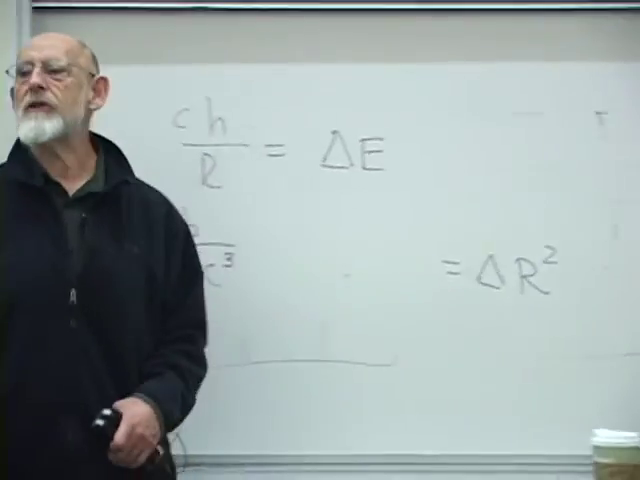
\includegraphics[width=0.84\textwidth]{lecture_02_figure_05.png}
\caption{黒板での完成したスケーリング議論。1ビットのエネルギー\(\Delta E\sim\hbar c/R_s\)は、\(G\hbar/c^3\)程度の半径の二乗、したがって面積の増分をもたらす。}
\lectureframe{01:22:40.000}
\end{figure}

実演計算の途中で\(c\)の因子が復元され、聴衆の一人がシュヴァルツシルト半径における欠落した\(c^{-2}\)を指摘する。その修正こそが式~\eqref{eq:planck-patch}における\(c^{-3}\)を生み出すものである。

\begin{classroomqa}
\audiencequestion{計算の一部だけで\(c\)を復元すると、その2乗を失うのか。\lecturetimestamp{01:21:18}}
\lecturerresponse{はい。次元関係は\(R_s=2GM/c^2\)であり、単に\(2GM\)ではない。その因子を復元すると面積は\(G\hbar/c^3\)のスケールになる。}
\end{classroomqa}

\(G\simeq6.7\times10^{-11}\,\mathrm{m^3\,kg^{-1}\,s^{-2}}\)、\(\hbar\simeq1.05\times10^{-34}\,\mathrm{J\,s}\)、\(c^3\simeq2.7\times10^{25}\,\mathrm{m^3\,s^{-3}}\)を用いると、
\begin{equation}
\ell_P^2\simeq2.6\times10^{-70}\,\mathrm{m^2},
\qquad
\ell_P\simeq1.6\times10^{-35}\,\mathrm{m}.
\end{equation}
黒板で見積もりを行う間、講義中の口頭の冪は揺れるが、物理的結論は安定している。このスケールは直接実験の分解能をはるかに下回る。

忘れがたいイメージは、鋭い肘をもつ不可侵のビットが地平線上に蓄積し、互いを押しのけ合うというものである。それぞれの新しいビットはおよそ1プランク面積のパッチを占める。これは面積の勘定のための比喩であって、文字どおりの正方形タイルが地平線を形成するという主張ではない。

\begin{classroomqa}
\audiencequestion{最初の光子がまだ近づいているときに、別の光子が地平線を拡大すると、古い光子は新しい地平線の内側に位置することになるのではないか。\lecturetimestamp{01:26:39}}
\lecturerresponse{単純な静的描像は、その問いを決着させるには十分に精密ではない。動的な時空における事象の地平線は大域的に定義されなければならず、その位置は物質が到着するにつれて変化する。ここで用いている外部記述では、情報は成長する地平線に関連づけられたままである。その地平線の厳密な定義は後回しにする。}
\end{classroomqa}

\begin{classroomqa}
\audiencequestion{巨大な質量が加えられる場合、たとえば二つのブラックホールが衝突する場合にも同じ問題が生じるのか。\lecturetimestamp{01:27:03}}
\lecturerresponse{はい。その場合には動的な性格を無視することは不可能である。講義では、地平線がより注意深く定義されるまで、合体の幾何学の完全な扱いを延期する。}
\end{classroomqa}

\begin{classroomqa}
\audiencequestion{プランク面積は、球面の地平線上ではなく、平らなパッチ上でのみ定義されるのか。\lecturetimestamp{01:27:30}}
\lecturerresponse{それは球面上の面積スケールであって、地平線が平らであることを要求するものではない。この数え上げにとって、平面か球面かという区別は重要ではない。}
\end{classroomqa}
\editorialnote{地平線の曲率半径が\(\ell_P\)に比べて巨大であるとき、各プランクサイズの近傍は局所的にほとんど平らである。}

直径八キロメートルの穴に対しては、限界の光子はそれに対応して、ほぼそのスケールの長い電波となる。聴衆向けの類推では、サイズに依存しない面積の増分を、バスケットボールの周りに巻いた紐にでも地球の周りに巻いた紐にでも同じ追加周長を加えることになぞらえている。どちらの場合も、固定された追加周長によって生じる半径方向の隙間は同じである。正確な幾何学は異なるが、どちらの例も、対象の元のサイズに依存しない変化を切り出している。

\section{面積の法則}

一度に1ビットずつ加えると、地平線の面積は普遍的な微視的量だけ変化する。したがって隠されうるビットの数は、体積ではなく\(A/\ell_P^2\)に比例しなければならない。ベッケンシュタインはこの比例関係を推論し、ホーキングの計算がその係数を確定した：
\begin{equation}
S_{\mathrm{BH}}=\frac{k_B A c^3}{4G\hbar}
=\frac{k_B A}{4\ell_P^2}.
\label{eq:bh-entropy}
\end{equation}
エントロピーを熱力学的単位ではなく二進ビットで数えるなら、\(S_{\mathrm{BH}}/k_B\)を\(\ln2\)で割る。

\begin{figure}[htbp]
\centering
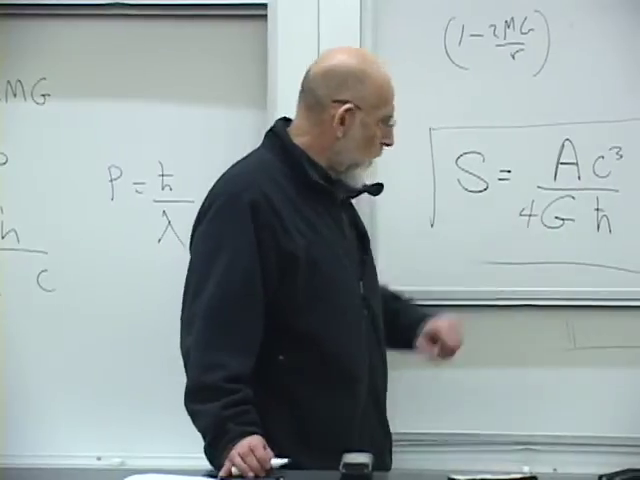
\includegraphics[width=0.84\textwidth]{lecture_02_figure_06.png}
\caption{ホーキングの因子\(1/4\)を含む最終的な板書の式は、講義のエントロピー単位で\(S\propto Ac^3/(4G\hbar)\)である。}
\lectureframe{01:31:02.000}
\end{figure}

したがってブラックホールは、同程度のサイズの通常の系よりも、桁違いに大きなエントロピーをもつ。それでもなお、その答えは素朴な体積の数え上げが示唆するよりも小さい。独立な情報は表面の測度によって制限される。この逆転---三次元の重力領域が二次元の境界としてスケールする情報によって記述されること---が、ホログラフィー原理の種である。

\begin{classroomqa}
\audiencequestion{エントロピーの式における因子\(1/4\)はどこから来るのか。\lecturetimestamp{01:30:30}}
\lecturerresponse{ベッケンシュタインの議論は面積への依存性と基本定数を確定したが、未知の係数を残した。彼の見積もりは2の対数などの可能性を生んだ。ホーキングの量子場の計算が係数を正確に\(1/4\)に確定した。}
\end{classroomqa}

\(\hbar\)の位置に最後の驚きが含まれている。量子エントロピーは\(\hbar\)に比例し、古典極限で消えると期待するかもしれない。そうではなく、\(\hbar\)が分母にある。\(\hbar\to0\)のとき、波は任意に小さいエネルギーコストで任意に細かい情報を運びうるので、エントロピー容量は発散する。量子化は、それ以外は古典的な穴に微小なエントロピーを加えるのではない。情報容量が無限になるのを防ぐのである。

\begin{classroomqa}
\audiencequestion{角運動量の単位をもつ\(\hbar\)が、通常の運動量と波長の関係も定めるのはなぜか。\lecturetimestamp{01:33:23}}
\lecturerresponse{\(\hbar\)は作用の単位、等価的には運動量×距離の単位をもつ。\(p\lambda\)が同じ単位をもつので、量子関係は\(2\pi\)の慣習を除いて\(p\sim\hbar/\lambda\)でありうる。角運動量\(\mathbf r\times\mathbf p\)が同じ次元をもつのは同じ理由による。}
\end{classroomqa}

講義はここで終わる。主題が尽きたからではなく、ここが正しい境界だからである。幾何学は地平線がなぜ情報を隠すのかを我々に告げ、熱力学は隠された情報をいかに数えるかを我々に告げ、量子力学はビット当たりの有限な面積を与えた。次の問いはもはや、ブラックホールが微視的状態を持つかどうかではなく、それらの状態が落下したものをどのように符号化し、最終的にどのように返すかである。